
In questa sezione ...

\section{Context-Awareness\label{sec:context-awareness}}

\textcolor{red}{STEFANO\\Informazioni storiche sulle ricerche relative al contesto} \cite{DBLP:journals/sigmod/BolchiniCQST07} \cite{baldauf2007survey}

\subsection{Context Dimension Model\label{sec:contex-dimension-model}}

\textcolor{red}{STEFANO\\Definizione del CDT}

In questa sezione verr� presentato il \emph{Context Dimension Tree} \cite{DBLP:journals/is/BolchiniQT13}, che � il modello di rappresentazione del contesto che verr� utilizzato in CAMUS. Il CDT � rappresentato come un albero $ \mathcal{T} = <N, E, r> $ ,composto da una radice e da nodi con etichetta, che descrive i possibili contesti nei quali ci si pu� trovare in una data situazione. \`E formato da una radice \emph{r} e un insieme di nodi \emph{N}, che vengono partizionati nei sottoinsiemi dei \emph{nodi dimensione} $N_D$, colorati di nero, e nei \emph{nodi concetto} $N_C$, colorati di bianco, che rappresentano i valori che possono assumere le dimensioni. La radice \emph{r} � un \emph{nodo concetto}, in quanto rappresenta il contesto pi� generale possibile, che corrisponde dunque all'intero dataset.

\begin{figure}[h]
	\centering
	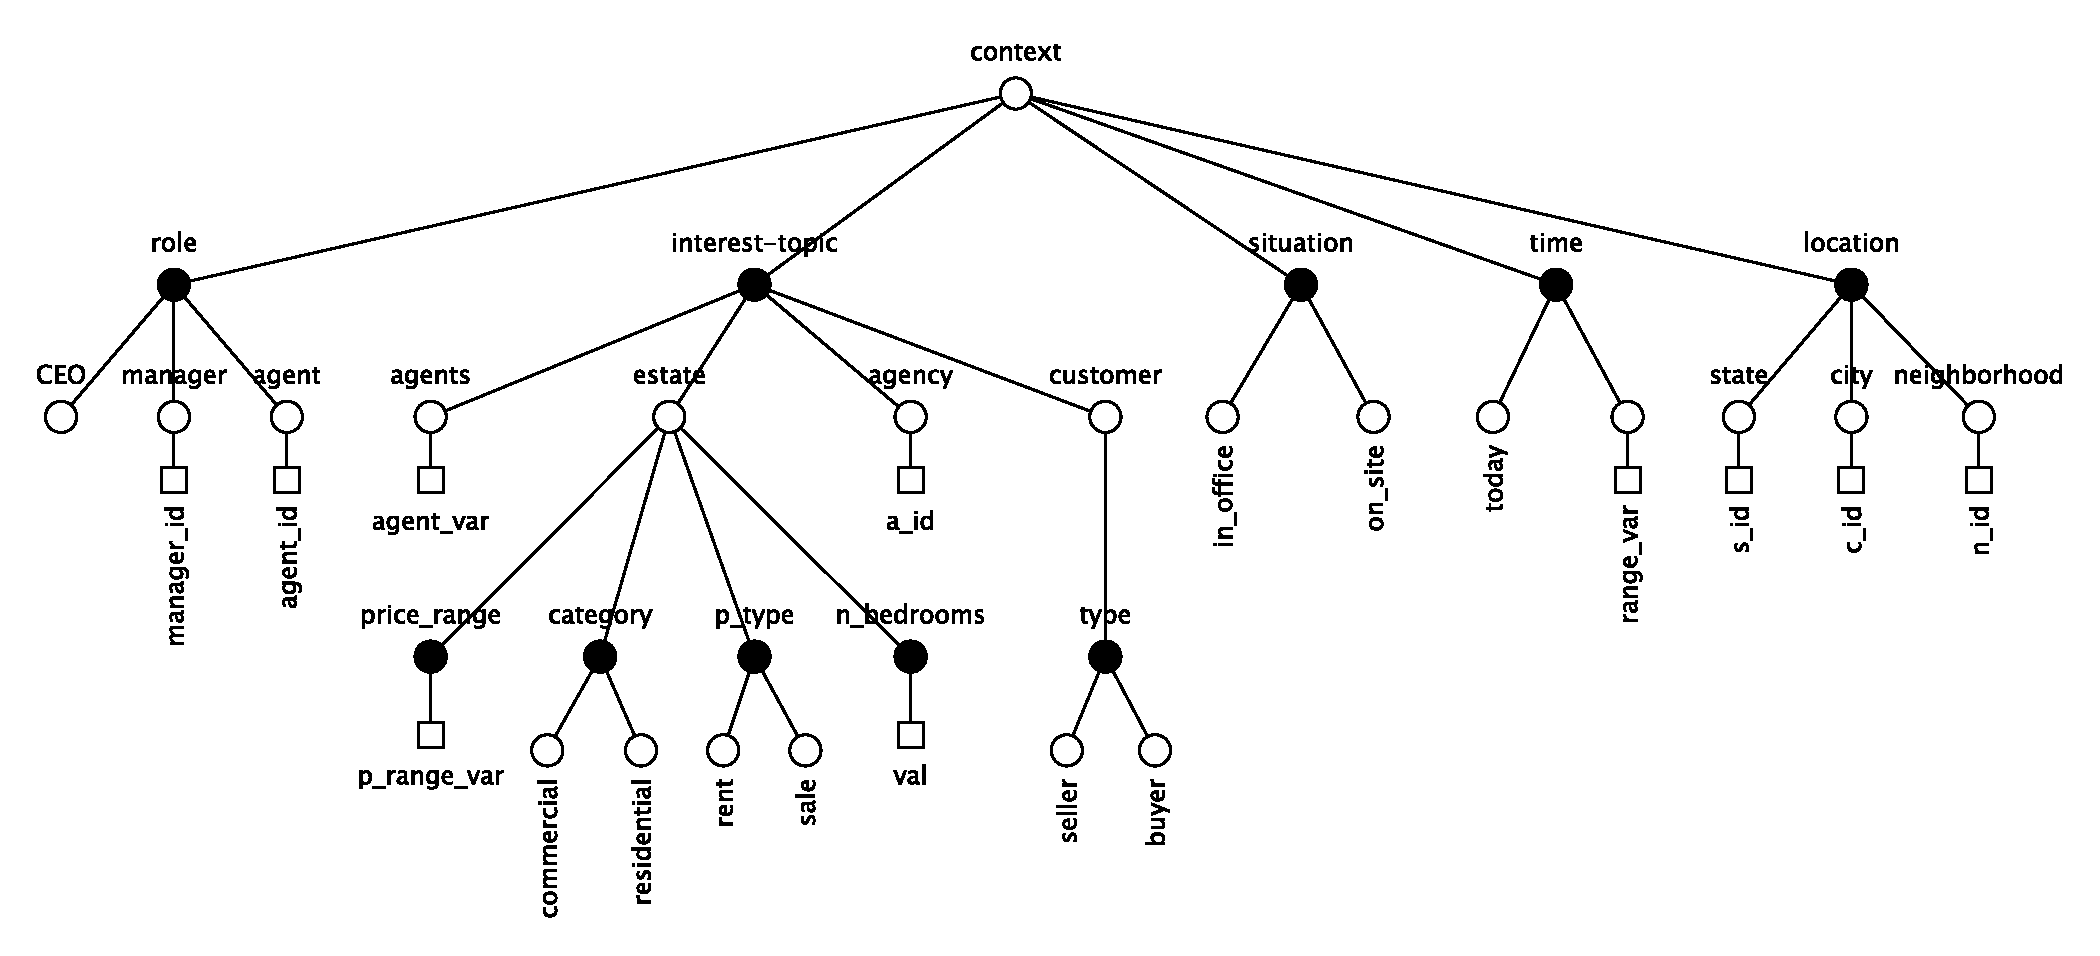
\includegraphics[width=\textwidth]{2-nozioni-preliminari/Immagini/esempio_cdt.png}
	\caption{Context Dimension Tree}\label{fig:context-dimension-tree}
\end{figure}

Le dimensioni che sono dirette discendenti della radice vengono chiamate \emph{dimensioni principali}, perch� definiscono le differenti caratteristiche dell'utente e del contesto nel quale agiscono. \textcolor{red}{aggiungere figura ed esempio} Inoltre, ogni valore pu� essere ulteriormente specializzato tramite \emph{sottodimensioni}, che a loro volta formano un sottoalbero. \textcolor{red}{aggiungere esempio}

Ogni nodo del CDT � caratterizzato dalla sua tipologia, che pu� essere \emph{dimensione} o \emph{concetto}, e dalla sua etichetta. Ogni nodo pu� essere identificato univocamente tramite l'unico percorso che lo collega alla radice. Senza perdita di generalit�, viene adottata l'ipotesi che ogni etichetta sia unica in un albero, quindi ogni nodo pu� essere identificato semplicemente dalla sua etichetta. I collegamenti tra i vari nodi non vengono invece etichettati.

L'alternanza tra nodi \emph{dimensione} e \emph{concetto} fa s� che vengano create delle \emph{generazioni}, ognuna delle quali sar� formata da nodi dello stesso colore, e ogni colore verr� alternato man mano che si prosegue discendendo nell'albero: dunque ogni \emph{nodo dimensione} pu� avere come figli solo nodi di tipo \emph{concetto} e viceversa.

\section{Mobile Mashup\label{sec:mobile-mashup}}

\textcolor{red}{VALERIO\\Informazioni generali sui mashup (non solo mobile)\\
Modello Visuale utilizzato\\
Sottosezione relativa a React Native (spiegare profonda integrazione con la piattaforma di riferimento e confronto con le webview)}

\section{Web Services\label{sec:web-services}}

\textcolor{red}{STEFANO\\Introduzione su cosa sono i servizi web\\
Caratteristiche dei servizi web (free, pagamento, paradigmi, ...)\\
Classificazione dei servizi esistenti (SOAP, REST, ...) e modi di interrogazione\\
Descrizione GraphQL, problemi che vuole risolvere e paragone con REST}

\section{Stato dell'arte\label{sec:stato-arte}}

\textcolor{red}{Descrizione dei principali "competitor" (IFTTT, Atooma, Swagger, Appery.io, Kimono, AdAPT, Yahoo Pipes, JackBe Presto, Mashart.org, Peudom)}